The device layer is the simplest layer in the system, and consist of the drivers for the SR300 and the interface for it.

\begin{figure}[h!]
	\centering
	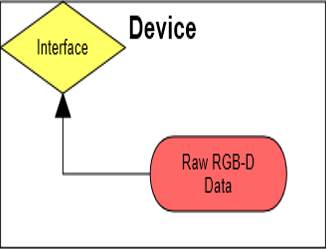
\includegraphics[width=0.60\textwidth]{images/device}
	\caption{Example subsystem description diagram}
\end{figure}

\subsection{Data}
The data subsystem only sends its data out to the interface.

\subsubsection{Subsystem Interfaces}

\begin {table}[H]
\caption {Subsystem interfaces} 
\begin{center}
    \begin{tabular}{ | p{1cm} | p{6cm} | p{3cm} | p{3cm} |}
    \hline
    ID & Description & Inputs & Outputs \\ \hline
    \#xx & Data/Interface & \pbox{3cm}{N/A} & \pbox{3cm}{Data Stream}  \\ \hline
    \end{tabular}
\end{center}
\end{table}

